% !TeX program = lualatex
% !TeX encoding = utf8
% !TeX spellcheck = uk_UA
% !BIB program = biber

\documentclass[]{beamer}
\usetheme{QuantumChemistry}
\usepackage{QuantumChemistry}

\addbibresource{../Bibliography/QuantumChemistry.bib}
\AtEveryCitekey{\clearfield{url}\clearfield{doi}}
\usetikzlibrary{chains, positioning}
\usepackage{ragged2e}
\usepackage{ifthen}
\graphicspath{{pictures/}}
\newcommand\vertarrowbox[3][6ex]{%
  \begin{array}[t]{@{}c@{}} #2 \\
  \left\uparrow\vcenter{\hrule height #1}\right.\kern-\nulldelimiterspace\\
  \makebox[0pt]{\scriptsize#3}
  \end{array}%
}

\usetikzlibrary{fadings,shapes.arrows,shadows}

\tikzfading[name=arrowfading, top color=transparent!0, bottom color=transparent!95]
\tikzset{arrowfill/.style={top color=gray!20, bottom color=white, general shadow={fill=black, shadow yshift=-0.8ex, path fading=arrowfading}}}
\tikzset{arrowstyle/.style={draw,arrowfill, single arrow,minimum height=1cm, single arrow}}

\newcommand{\tikzfancyarrow}[1]{\tikz[baseline=-0.5ex]\node [arrowstyle] {#1};}

\usepackage{pdfpages}
\title[Лекції з квантової хімії]{\huge\bfseries Рівняння Хартрі-Фока}
\subtitle{Лекції з квантової хімії}
\author{Пономаренко С. М.}
\date{}

\begin{document}
%=======================================================================================================
\usebackgroundtemplate{
	\tikz\node[opacity=0.15]{\includegraphics[width=\paperwidth,height=\paperheight]{background}};%
}
\begin{frame}
    \thispagestyle{empty}
	\titlepage
\end{frame}
%=======================================================================================================


%%============================================================================
%\begin{frame}{Зміст}{}
%	\tableofcontents
%\end{frame}
%%============================================================================



%\section{Задача}
%============================================================================
\begin{frame}{П. А. М. Дірак}{1928, релятивістське рівняння руху електрона (ферміонів)}
	\begin{columns}
		\begin{column}{.3\linewidth}
			\begin{center}
				\includegraphics[width=1\linewidth]{Dirac}
			\end{center}
		\end{column}
		\begin{column}{0.7\linewidth}
			\begin{equation*}
				\tcbhighmath[drop fuzzy shadow]{i\hbar \gamma ^{\mu }\partial _{\mu }\psi -mc\psi =0}
			\end{equation*}
			\begin{quote}\small
				\rmfamily <<Нарешті, основні фізичні закони  необхідні для побудови математичної теорії здебільшого фізики і всієї хімії, повністю відомі, і єдина складність полягає в тому, що в результаті застосування цих законів ми приходимо до дуже складних для розв'язання рівнянь>>
			\end{quote}
		\end{column}
	\end{columns}
	\begin{center}\footnotesize
		Dirac P.A.M. Quantum Mechanics of Many Electron Systems // Proceedings of the Royal Society A123 (1929): 713.
	\end{center}
\end{frame}
%============================================================================
\begin{frame}[t]{Гамільтоніан електронної підсистеми системи}

	\begin{multline*}
		\hat{H}_e = \hat{T}_{e} + \hat{V}_{en} + \hat{V}_{ee} + \ldots = \\ = -\frac12 \sum\limits_{i}^{N_e} \vec{\nabla}^2_i - \sum\limits_\alpha^{N_n}\sum\limits_{i}^{N_e} \frac{Z_\alpha}{r_i} + \frac12 \sum\limits_{i}^{N_e}\sum\limits_{\substack{j,\, j \neq i}}^{N_e}\frac{1}{r_{ij}}+\\ + \sum\limits_{\alpha}\sum\limits_{\beta, \alpha \neq \beta}\frac{Z_\alpha Z_\beta}{R_{\alpha\beta}} + \\ + \hat\varepsilon_{Orb-Spin} + \hat\varepsilon_{Spin-Spin} +\hat\varepsilon_{Orb-Orb},
	\end{multline*}
\end{frame}
%============================================================================
%============================================================================
\begin{frame}{Задача}{}
	Необхідно розв'язати електронне рівняння Шредінґера:
	\begin{equation*}
		\tcbhighmath{\hat{H}_e \Phi(\vxi) = E_e(\vec{R})\Phi(\vxi)}
	\end{equation*}
	знайшовши хвильову функцію всіх $N_e$ електронів, що у нас є, і їх енергію в полі ядер.
	Хвильова функція у нас залежить
	\begin{itemize}
		\item від $3N_e$ просторових змінних $\vec{r} = (\vec{r}_1, \vec{r}_2,\ldots, \vec{r}_{N_e})$, що описують стан кожного електрона в просторі;
		\item від  $N_e$ ступенів свободи, що описують орієнтацію спінів електронів в просторі $\sigma = (\sigma_1, \sigma_2, \ldots, \sigma_{N_e})$.

			      {\scriptsize Спінові змінні відрізняються від просторових тим, що вони відсутні в електронному гамільтоніані, тобто ніякого вкладу в енергію в нашому наближенні вони не вносять. }
	\end{itemize}

	В підсумку ми маємо $4N_e$ ступенів свободи:
	\[
		\vxi = (\underbrace{\vec{r}_1, \sigma_1}_{\xi_1}, \underbrace{\vec{r}_2, \sigma_2}_{\xi_2}, \ldots, \underbrace{\vec{r}_{N_e}, \sigma_{N_e}}_{\xi_{N_e}})
	\]
\end{frame}
%============================================================================

%\section{Одноелектронне наближення. Детермінант Слейтера}

%============================================================================
\begin{frame}{Принцип Паулі}{сформульовано Вольфгангом Паулі 1925 року }
	\begin{columns}
		\begin{column}{0.4\linewidth}
			\begin{center}
				\includegraphics[width=0.75\linewidth]{Pauli}
			\end{center}
		\end{column}
		\begin{column}{0.6\linewidth}
			\begin{block}{}\small
				Система частинок з напівцілими спінами, --- система ферміонів, --- має описуватися хвильовою функцією, яка змінює знак при перестановці координат і спінових змінних будь-якої пари. Під перестановкою місцями розуміють <<обмін>> як просторовими, так і спіновими змінними будь-яких двох частинок. Тобто функція має бути \textit{антисиметричною} по відношенню до перестановки місцями двох довільних електронів, наприклад $i$-го і $j$-го:
				\begin{multline*}
					\Phi (\xi_1, \xi_2, \ldots, \xi_i, \ldots \xi_j, \ldots, \xi_{N_e}) = \\ = - \Phi (\xi_1, \xi_2, \ldots, \xi_j, \ldots \xi_i, \ldots, \xi_{N_e})
				\end{multline*}
			\end{block}
		\end{column}
	\end{columns}
\end{frame}
%============================================================================

%============================================================================
\begin{frame}{Система невзаємодіючих частинок}{Представлення Хартрі}

	Якби електронний гамільтоніан мав вигляд (без електрон-електронної взаємодії):
	\begin{equation*}\label{}
		\hat{H}_e = \sum\limits_{i = 1}^{N_e}\left(-\frac12\nabla_i^2 + \sum\limits_{\alpha =1}^{N_n}\frac{Z\alpha}{r_i}\right) = \sum\limits_{i = 1}^{N_e} \hat{h}_i,
	\end{equation*}
	хвильову функцію для всіх електронів можна було представити у вигляді:
	\begin{equation*}
		\Phi(\vxi) = \prod\limits_{i = 1}^{N_e} \vphi_{k_i}(\vxi_i),
	\end{equation*}
	Представлення багатоелектронної хвильової функції виражається через добуток одноелектронних називається \emph{представленням Хартрі}.

	\medskip

	\begin{center}
		\alert{Не враховується симетрія хвильової функції $\Rightarrow$ суперечить принципу Паулі}
	\end{center}
\end{frame}
%============================================================================

%============================================================================
\begin{frame}{Хвильова функція невзаємодіючих частинок}{Орбіталі}

	Одноелектронна функція називається \alert{спін-орбіталлю}, оскільки вона залежить як від спінових змінних $\sigma$  так і від просторових координат~$\vec{r}$.

	\begin{equation*}\label{spin-orbit}
		\vphi_i(\vec{r}_i, \sigma_i),
	\end{equation*}


	Так як гамільтоніан не враховує спін-орбітальну взаємодію, то спін-орбіталь в свою чергу можна представити у вигляді добутку координатної та спінової функцій:
	\begin{equation*}
		\vphi_i(\vec{r}_i, \sigma_i) = \phi_i(\vec{r}_i) \gamma_i(\sigma_i), \quad \text{де } \gamma = \alpha (\text{ або }\uparrow), \beta (\text{ або }\downarrow)
	\end{equation*}
	Координатна функція $\phi_i(\vec{r}_i)$ називається \alert{орбіталлю}.

	\begin{overprint}
		\onslide<1>
		Кожна спін-орбіталь нормована на одиницю
		\begin{equation*}
			\bracket{\vphi_i}{\vphi_i} = \int \vphi_i^*(\vec{r}_i, \sigma_i) \vphi_i(\vec{r}_i, \sigma_i) dx_idy_idz_id\sigma_i = 1
		\end{equation*}
		\onslide<2>
		Для спінових частин
		\begin{equation*}\label{}
			\bracket{\alpha}{\alpha} = \bracket{\beta}{\beta} = \int \alpha^*(\sigma) \alpha(\sigma) d\sigma = 1, \, \bracket{\alpha}{\beta} = \int \alpha^*(\sigma) \beta(\sigma) d\sigma = 0.
		\end{equation*}
	\end{overprint}
\end{frame}
%============================================================================






%============================================================================
\begin{frame}{Детермінант Слейтера}{}
	У випадку $N_e$ невзаємодіючих частинок:
	\begin{equation*}\label{DetSlat}
		\begin{gathered}
			\Phi (\vxi_1, \vxi_2,\ldots,\vxi_{N_e})= {\frac {1}{\sqrt {N_e!}}} = \\ =
			\left|
			{
			\begin{matrix}
				\vphi_{1}(\vxi_1) & \vphi_{1}(\vxi_2) & \ldots & \vphi_{1}(\vxi_{N_e}) \\
				\vphi_{2}(\vxi_1) & \vphi_{2}(\vxi_2) & \ldots & \vphi_{2}(\vxi_{N_e}) \\
				\vdots            & \vdots            & \vdots & \vdots                \\
				\vphi_{N}(\vxi_1) & \vphi_{N}(\vxi_2) & \ldots & \vphi_{N}(\vxi_{N_e})
			\end{matrix}
			}
			\right| = {\frac {1}{\sqrt {N_e!}}} \sum\limits_{\vec{k}} (-1)^{p(\vec{k})} \prod\limits_{i = 1}^{N_e} \vphi_{k_i}(\vxi_i),
		\end{gathered}
	\end{equation*}
	де $\vec{k} = \{k_1,k_2, \ldots, k_{N_e}\}$ --- набір перестановок, а $p(\vec{k})$~--- парність цих перестановок ($+1$~--- для парних, $-1$~--- для непарних).
    	\begin{myexample}{\small Принцип заборони Паулі}\small
        Одну орбіталь можуть займати не більш як два електрони з антипаралельними спінами.
    \end{myexample}
\end{frame}
%============================================================================

%============================================================================
%\begin{frame}{Як виглядає справжня багатоелектронна $\Phi$?}{}
%	Всі можливі функції, що задаються набором спін-орбіталей, ми теж можемо пронумерувати:
%	\begin{equation*}\label{}
%		\Phi_n = \frac{1}{\sqrt{N_e!}} = \mathrm{det} \{\phi^{(n)}_1, \phi^{(n)}_2, \ldots, \phi^{(n)}_{N_e}\},
%	\end{equation*}
%	вони утворюють повний ортонормований базис:
%	\begin{equation*}\label{}
%		\bracket{\Phi_n}{\Phi_m} = \delta_{nm},
%	\end{equation*}
%	оскільки є власними функціями гамільтоніана невзаємодіючих частинок.
%
%\begin{block}{}\justifying
%    	Детермінант Слейтера --- це конструкція, за допомогою якої тепер можна організувати зручне представлення для справжньої багатоелектронної функції у вигляді розкладання в ряд по ним:
%	\begin{equation*}\label{}
%		\Phi_e = \sum\limits_{n = 1}^\infty \Phi_n.
%	\end{equation*}
%\end{block}
%\end{frame}
%============================================================================




%============================================================================
\begin{frame}[t]{Варіаційний принцип}{}
    %----------------------------------------------------------------------------
    \begin{tblr}{cc}
        Енергія системи в в квантовій механіці
        &
        \(
        E[\Phi]  = \dfrac{\opbracket{\Phi}{\hat{H}}{\Phi}}{\bracket{\Phi}{\Phi}}
        \)
        \\
    \end{tblr}
    %    \begin{columns}[c]
        %        \begin{column}{0.5\linewidth}
            %            	Енергія системи в в квантовій механіці
            %        \end{column}
        %        \begin{column}{0.5\linewidth}
            %            	\[
            %            \tcbhighmath{
                %                E[\Phi]  = \dfrac{\opbracket{\Phi}{\hat{H}}{\Phi}}{\bracket{\Phi}{\Phi}}
                %            }
            %            \]
            %        \end{column}
        %    \end{columns}



    \begin{alertblock}{}\small\centering
        Енергія системи --- функціонал від функції стану $\Phi$ системи!
    \end{alertblock}
    %\begin{flushleft}\scriptsize\justifying
    %        Одним з найбільш витончених способів висловити умови, що виділяють із усіх можливих функцій $\Phi$, ті, які описують нашу систему --- є принцип мінімуму функціоналу енергії.
    %\end{flushleft}
    \begin{myexample}{Варіаційний принцип}\justifying
        \begin{tblr}{X[j,m]Q}
            Справжні функції, які описують систему отримують є розв'язками диференціальних рівнянь, які можна отримати із умови мінімуму функціоналу енергії.
            &
            $\delta E[\Phi] = 0$
            \\
        \end{tblr}
    \end{myexample}



    \begin{onlyenv}<1>
        \scriptsize
        %	Застосуємо варіаційний принцип $\delta E = 0$
        %	\[
        %		\delta E =  \int \delta \Phi^* \hat{H} \Phi d\xi + \int \Phi^* \hat{H} \delta \Phi d\xi = 0
        %	\]
        Разом з варіацією умови нормування  $\delta \int \Phi^*  \Phi d\xi = 0$  (метод невизначених множників Лагранжа)
        %	\[
        %		\delta \left(-\lambda \int \Phi^*  \Phi d\xi - 1\right)=  -\lambda \int \delta \Phi^* \Phi d\xi -\lambda  \int  \Phi -^*  \delta \Phi d\xi = 0
        %	\]
        \[
        \int \delta \Phi^* \left( \hat{H} - \lambda\right) \Phi d\xi + \int \delta \Phi \left( \hat{H} - \lambda\right)^{\dagger} \Phi^* d\xi = 0  \rightarrow \hat{H}  \Phi = \lambda  \Phi, \lambda = E
        \]
        варіація функціоналу енергії дає нам рівняння Шредінґера.
    \end{onlyenv}

    \begin{onlyenv}<2>
        \begin{alertblock}{}\centering\footnotesize
            Якщо на хвильову функцію не накладати жодних умов (крім умови нормування) ---  варіаційний принцип еквівалентний розв'язуванню  рівняння Шредінґера.
        \end{alertblock}
    \end{onlyenv}
    %	\begin{alertblock}{}\centering\small
        %		\alert{Зазвичай ми не знаємо точну функцію!}
        %%	\end{alertblock}
    %\begin{alertblock}{}\centering\small
    %    Ми не можемо розв'язувати рівняння Шредінґера для систем з числом електронів більше одного!
    %\end{alertblock}
\end{frame}
%============================================================================




%============================================================================
\begin{frame}{Одноелектронне наближення}{}
    \begin{myexample}{Одноелектронне наближення}\small\justify
        \begin{tblr}{X[j,m]Q[c,m]}
            Квантову систему \emphs[red]{наближено} можна описати як систему окремих \emphs[red]{незалежних електронів}. Кожен електрон рухається потенціальному полі ядер і усередненому полі інших електронів.
            &
            %			\begin{center}
                \tikz[scale=0.5, baseline]{
                    \path[inner color=red, outer color=white] (0,0) circle(2.5);
                    \fill[ball color=blue!50] (0,0) circle (0.4);
                    \fill[ball color=red!50]  (45:1.5) coordinate (E2) circle (0.1);
                }
                %			\end{center}
            \\
        \end{tblr}
    \end{myexample}
    Плюси цієї моделі:
    \begin{enumerate}[\faHandORight]
        \item Кожен електрон описується своєю орбіталлю.
        \item Хвильову функцію системи електронів можна описати як функцію незалежних частинок --- у вигляді \emphs[red]{одного єдиного детермінанту Слейтера}.
    \end{enumerate}
    \begin{alertblock}{}
        Рівняння для орбіталей можна знайти з варіаційного принципу.
    \end{alertblock}
\end{frame}
%============================================================================





%============================================================================
\begin{frame}{Варіаційний теорема}{}
    \begin{myexample}{Варіаційна теорема}
        \begin{tblr}{X[j, m]Q}
            При довільному виборі хвильової функції $\tilde{\Phi}$ середнє значення
            енергії $E$ завжди буде обмеженим знизу точним значенням енергії відповідного стаціонарного стану $E_0$.
            &
            $E_0 \le E = \opbracket{\tilde{\Phi}}{\hat{H}}{\tilde{\Phi}}$
            \\
        \end{tblr}
    \end{myexample}
    %\begin{exampleblock}\scriptsize
    %        Наближену функції системи $\tilde{\Phi}$ можна представити у вигляді розкладання
    %    \[
    %        \tilde{\Phi} = \sum\limits_m C_m\Phi_m,
    %    \]
    %    $\Phi_m$ є власними функціями точного гамільтоніана системи $\hat{H} \Phi_m = E_m \Phi_m$.
    %
    %    Енергія системи, розрахована для наближеної функції $\tilde{\Phi}$
    %
    %    \begin{equation*}
        %            E  = \opbracket{\tilde\Phi}{\hat{H}}{\tilde\Phi} = \sum\limits_m |C_m|^2 E_m.
        %        \end{equation*}
    %
    %    Нехай $E_0$ найменше  значення енергії основного стану системи, тоді
    %    \begin{equation*}
        %            E  = \opbracket{\tilde\Phi}{\hat{H}}{\tilde\Phi} = \sum\limits_m |C_m|^2 E_m \ge \sum\limits_m |C_m|^2 E_0  = E_0.
        %        \end{equation*}
    %\end{exampleblock}

    \begin{block}{}\centering
        Енергія обчислена за наближеною функцією $\tilde\Phi$  буде оцінкою зверху для точного значення енергії основного стану системи:
        \[
        E_{\min} \ge E_0
        \]
    \end{block}

    \begin{alertblock}{}\centering
        Енергія системи, знайдена в одноелектронному наближені буде більше точного значення енергії основного стану системи.
    \end{alertblock}
\end{frame}
%============================================================================





%============================================================================
%\section{Рівняння Хартрі-Фока}
\begin{frame}{Правила Слейтера}{Без виведення}
	\begin{overprint}
		\onslide<1>
		Середнє значення одночастинкового оператора $\hat{A} = \sum\limits_{l= 1}^{N_e} \hat{a}_l$.

		Діагональний елемент:
		\begin{equation*}\label{}
			\opbracket{\Phi_n}{\hat{A}}{\Phi_n} = \sum\limits_{i = 1}^{N_e} \opbracket{\vphi_{k_i}(\vxi)}{\hat{a}}{\vphi_{k_i}(\vxi)}
		\end{equation*}
		дорівнює сумі діагональних елементів спін-орбіталей функцій з набору, на якому побудований детермінант Слейтера.

		%     Якщо $\Phi_n$ відрізняються бодай на одну функцію:
		%	\begin{equation*}\label{}
		%		\opbracket{\Phi_n}{\hat{A}}{\Phi_m} = 0
		%	\end{equation*}
		В скороченому вигляді
		\begin{equation*}\label{}
			\opbracket{\vphi_{k_i}(\vxi)}{\hat{a}}{\vphi_{k_i}(\vxi)} = \opbracket{i}{\hat{a}}{j}
		\end{equation*}
		\onslide<2>
		Середнє значення двочастинкового оператора $\hat{B} = \frac12\sum\limits_{j= 1}^{N_e} \sum\limits_{j, j\neq i}^{N_e}\hat{b}_{ij}$.

		Діагональний елемент:
		\begin{multline*}\label{}
			\opbracket{\Phi_n}{\hat{B}}{\Phi_n} = \frac12\sum\limits_{i = 1}^{N_e} \sum\limits_{j = 1, j \neq 1}^{N_e} \left(
			\opbracket{\vphi_{k_i}(\vxi) \vphi_{k_j}(\vxi')  }{\hat{b}(\vxi,\vxi')}{\vphi_{k_i}(\vxi)\vphi_{k_j}(\vxi')} \right.+ \\ +
			%
			\left.
			\opbracket{\vphi_{k_i}(\vxi) \vphi_{k_j}(\vxi')  }{\hat{b}(\vxi,\vxi')}{\vphi_{k_j}(\vxi)\vphi_{k_i}(\vxi')}
			\right)
		\end{multline*}
		В скороченому вигляді
		\begin{multline*}\label{}
			\opbracket{\vphi_{k_i}(\vxi) \vphi_{k_j}(\vxi')  }{\hat{b}(\vxi,\vxi')}{\vphi_{k_i}(\vxi)\vphi_{k_j}(\vxi')} - \\ -
			%
			\opbracket{\vphi_{k_i}(\vxi) \vphi_{k_j}(\vxi')  }{\hat{b}(\vxi,\vxi')}{\vphi_{k_j}(\vxi)\vphi_{k_i}(\vxi')} = \bracket{ij}{ij} - \bracket{ij}{ji}
		\end{multline*}
	\end{overprint}
\end{frame}
%============================================================================

%============================================================================
%\begin{frame}{Рівняння Хартрі-Фока}{Однодетермінантне наближення}
%%	Справжню багатоелектронну функцію у вигляді розкладання в ряд по Детермінантам Слейтера:
%%	\begin{equation*}\label{}
%%		\Phi_e = \sum\limits_{n = 1}^\infty \Phi_n.
%%	\end{equation*}
%
%	Мінімально простою апроксимацією буде випадок \alert{однодетермінантного представлення}:
%	\begin{equation*}\label{}
%		\Phi_e \approx \Phi_0 = \mathrm{det}\{\vphi_1, \vphi_2, \ldots, \vphi_{N_e}\}.
%	\end{equation*}
%	Будемо застосовувати варіаційний принцип до виразу
%	\begin{equation*}\label{*}
%		E[\Phi_0] = \opbracket{\Phi_0}{\hat{H}_e}{\Phi_0}, \quad \delta E = 0
%	\end{equation*}
%	щоб отримати рівняння на електронну хвильову функцію.
%\end{frame}
%============================================================================

%============================================================================
\begin{frame}[t]{Рівняння Хартрі-Фока}
	\framesubtitle<1>{Що будемо варіювати?}
	\framesubtitle<2>{Одночастинковий та двочастинкові інтеграли}
	\framesubtitle<3>{Процедура варіювання}
	\only<1>{
		Гамільтоніан
		\begin{equation*}\label{}
			\hat{H}_e = \sum\limits_{i = 1}^{N_e} h_i + \frac12\sum\limits_{i}^{N_e}\sum\limits_{\substack{j=1, j \neq i}}^{N_e}\frac{1}{r_{ij}}
		\end{equation*}

\begin{alertblock}{}\centering
            Обираємо одноелектронне (однодетермінантне) наближення:
            \begin{equation*}\label{}
            	\Phi_e \approx \Phi_0 = \mathrm{det}\{\vphi_1, \vphi_2, \ldots, \vphi_{N_e}\}.
            \end{equation*}

\end{alertblock}
		Записуємо функціонал енергії і використаємо правила Слейтера:
		\begin{multline*}\label{}
			E[\Phi_0] = \opbracket{\Phi_0}{\hat{H}_e}{\Phi_0} = \sum\limits_{i = 1}^{N_e}   \opbracket{i}{\hat{h}_i}{i}_{\vxi} + \\ + \frac12\sum\limits_{i = 1}^{N_e} \sum\limits_{j = 1, j \neq i}^{N_e} \left( \opbracket{ij}{\frac1{r_{ij}}}{ij}_{\vxi, \vxi'} - \opbracket{ij}{\frac1{r_{ij}}}{ji}_{\vxi, \vxi'}\right)
		\end{multline*}
	}
	\only<2>
	{
		Одночастинковий інтеграл
		\(h_i= \int \vphi_i(\vxi_i) \hat{h}_i  \vphi_i(\vxi_i)  d\xi\)

		Кулонівський інтеграл
		\[J_{ij} = \opbracket{ij}{\frac1{r_{ij}}}{ij}_{\vxi, \vxi'} = \iint \vphi_i(\vxi) \vphi_j(\vxi') \frac1{r_{ij}}  \vphi_i(\vxi) \vphi_j(\vxi') d\xi d\xi',\]
		Обмінний інтеграл
		\[K_{ij} = \opbracket{ij}{\frac1{r_{ij}}}{ji}_{\vxi, \vxi'} = \iint \vphi_i(\vxi) \vphi_j(\vxi') \frac1{r_{ij}}  \vphi_j(\vxi) \vphi_i(\vxi') d\xi d\xi'.\]
		\begin{equation*}\label{*}
			\tcbhighmath{E[\Phi_0] = \opbracket{\Phi_0}{\hat{H}_e}{\Phi_0} = \sum\limits_{i = 1}^{N_e}   h_i + \frac12\sum\limits_{i = 1}^{N_e} \sum\limits_{j = 1, j \neq i}^{N_e} \left( J_{ij} - K_{ij}\right).}
		\end{equation*}
	}
	\only<3>{
		\[
			\Phi_0 + \delta_k\Phi_0 = \frac1{\sqrt{N_e!}}\mathrm{det}\{\vphi_1, \vphi_2, \ldots, \vphi_k + \delta\vphi_k, \ldots, \vphi_{N_e}\}
		\]
		\begin{equation*}\label{}
			\delta E[\Phi_0] = \opbracket{\delta_k\Phi_0}{\hat{H}_e}{\Phi_0} - \opbracket{\Phi_0}{\hat{H}_e}{\Phi_0} +\ldots
		\end{equation*}
		Але однієї варіації енергії нам не достатньо, тому треба накласти додаткові умови на наші спін-орбіталі, а саме вимогу ортогональності:
		\begin{equation*}\label{}
			L = \sum\limits_{i = 1}^{N_e} \sum\limits_{j = 1, j \neq i}^{N_e} \varepsilon_{ij} (\bracket{i}{j} -\delta_{ij}),
		\end{equation*}
		де $ \varepsilon_{ij}$~--- невизначені множники Лагранжа:
		\begin{equation*}\label{}
			\delta_k L = \sum\limits_{j = i}^{N_e}\varepsilon_{kj} \bracket{\delta k}{j} = 0 ,
		\end{equation*}
	}
	\only<4-5>{
		\begin{multline*}\label{}
			\opbracket{\delta k}{\hat{h}}{k} + \sum\limits_{j = 1, j \neq k}^{N_e} \left( \opbracket{\delta k j}{\frac1r}{kj} - \opbracket{\delta k j}{\frac1r}{jk}\right) - \\ - \sum\limits_{k = 1}^{N_e}\varepsilon_{kj} \bracket{\delta k}{j} = 0
		\end{multline*}
		Винесемо $\bra{\delta k} = \int \delta\vphi_k d\xi_k$ за дужки і отримаємо:
		\begin{equation*}\label{}
			\hat{h}\vphi_k(\vxi) + \sum\limits_{j = 1, j \neq k}^{N_e} \left( \opbracket{j}{\frac1r}{kj}_{\vxi'} - \opbracket{ j}{\frac1r}{jk}_{\vxi'}\right) \vphi_k(\vxi) =  \sum\limits_{j = i}^{N_e}\varepsilon_{kj} \vphi_j(\vxi) .
		\end{equation*}
		\begin{overprint}
			\onslide<4>
			Кулонівський оператор
			{\small\[
				\hat{J}_j \vphi_k(\vxi) = \opbracket{j}{\frac1r}{kj}_{\vxi'}  =  \left( \int \vphi_j(\vxi') \frac{1}{r} \vphi_j(\vxi') d\xi'\right) \cdot \phi_k(\vxi) .
			\]}
			\onslide<5>
			Обмінний оператор
			{\small \[
				\hat{K}_j \vphi_k(\vxi) =  \opbracket{j}{\frac1r}{jk}_{\vxi'}  =  \left( \int \vphi_j(\vxi') \frac{1}{r} \vphi_k(\vxi') d\xi'\right) \cdot \phi_j(\vxi) .
			\]}
		\end{overprint}
	}
	\only<6>{
		\begin{equation*}\label{}
			\hat{h}\vphi_k(\vxi) + \sum\limits_{j = 1, j \neq k}^{N_e} \left( J_j(\vxi') - K_j(\vxi')\right) \vphi_k(\vxi) =  \sum\limits_{j = i}^{N_e}\varepsilon_{kj} \vphi_j(\vxi) .
		\end{equation*}

		Використаємо той факт, що за допомогою унітарного перетворення всередині набору функцій $\{\vphi_1, \vphi_2,\ldots, \vphi_{N_e}\}$, ми можемо діагоналізувати матрицю $\varepsilon_{kj}$ при цьому не зіпсувавши ліву частина рівняння. А значить в правій частині буде стояти тільки $\varepsilon_{kk} \vphi_k =  \varepsilon_k \vphi_k$.
		\begin{equation*}\label{}
			\left(\hat{h} + \sum\limits_{j = 1, j \neq k}^{N_e} \left( \hat J_j(\vxi') - \hat K_j(\vxi')\right) \vphi_k(\vxi) \right)\vphi_k(\vxi)=  \varepsilon_{k} \vphi_k(\vxi) .
		\end{equation*}
	}
	\framesubtitle<7>{Канонічний вигляд рівнянь Хартрі-Фока}
	\only<7>{%
		\begin{equation*}\label{}
			\left(\hat{h} + \sum\limits_{j = 1, j \neq k}^{N_e} \left( \hat{J}_j - \hat{K}_j\right) \vphi_k(\vxi) \right)\vphi_k(\vxi)=  \varepsilon_{k} \vphi_k(\vxi) , \quad k =1, \ldots, N_e
		\end{equation*}
		або
	}%
	\only<7-8>{%
		\begin{equation*}\label{}
			\tcbhighmath{\hat{F}_k\vphi_k(\vxi)=  \varepsilon_{k} \vphi_k(\vxi),}
		\end{equation*}
		$\hat{F}_k$~--- фокіан (оператоор Фока).
	}%
	\only<7>{%
		\begin{alertblock}{}\centering
			Рівняння Хартрі-Фока ---  одне из головних рівнянь квантової хімії!
		\end{alertblock}
	}%
	\framesubtitle<8>{Фізичний смисл отриманих рівнянь}
	\only<8>%
	{%

	Наближення Хартрі-Фока зводиться до апроксимації точного електронного гамільтоніана $\hat{H}$ сумою одноелектронних операторів операторів Фока:
	\begin{equation*}\label{}
		\hat{H}_e \to \hat{\tilde{H}}_e = \sum\limits_{i = 1}^{N_e} \hat{F}_i = \sum\limits_{i = 1}^{N_e}\left(\hat{h}_i + \hat{V}_i \right),
	\end{equation*}
	де оператори $ \hat{V}_i $ визначаються середнім електростатичним полем, яке діє на кожен електрон з боку всіх інших електронів системи.

	\begin{block}{}\scriptsize
        Це додаткове поле є самоузгодженим, тобто змінюється при зміні стану електрона, що знаходиться в цьому полі.
    \end{block}

	}%
	\framesubtitle<9-10>{Канонічні орбіталі. Віртуальні орбіталі. Aufbau принцип}
	\only<9-10>%
	{%
		\begin{block}{Канонічні орбіталі}
			Орбіталі, одержувані при розв'язку рівнянь Хартрі-Фока називають канонічними.
		\end{block}
	}%
	\only<9-10>{%
		\begin{columns}
			\begin{column}{0.7\linewidth}\justifying
				\only<9>{%
					Число розв'язків рівнянь Хартрі-Фока в загальному випадку  нескінченно велике.\\~\\

					В якості спін-орбіталей, що займають електронами, зазвичай вибирають $N$ розв'язків канонічних рівнянь Хартрі-Фока, що відповідають найменшим енергій орбіталей і з них будують детермінант Слейтера. Всі інші орбіталі, які виявились незайнятими --- називають \alert{віртуальними орбіталями}.}%
				\only<10>{%

					Орбіталь, яка серед заповнених в основному стані має найбільшу енергію позначається абревіатурою ВЗМО (вища зайнята молекулярна орбіталь) або частіше англійською абревіатурою HOMO (highest occupied molecular orbital).
					\\~\\
					Наступна по енергії орбіталь називається НВМО (нижча вакантна молекулярна орбіталь) або LUMO (lowest unoccupied molecular orbital --- нижча незаповнена молекулярна орбіталь).
				}%
			\end{column}
			\begin{column}{0.3\linewidth}
				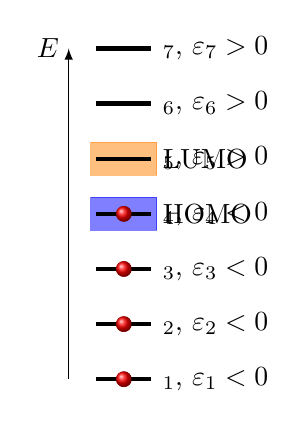
\begin{tikzpicture}[scale=0.7,
						upspinarrow/.pic = {\draw[-latex, blue] (0,-0.5) -- (0, 0.5);},
						downspinarrow/.pic = {\draw[latex-,red] (0,-0.5) -- (0, 0.5);},
						electron/.pic = {\node[circle, ball color = red, inner sep=2pt] {};},
					]
					\draw<10>[fill=blue, blue, opacity=0.5] (-0.1,3.7) rectangle ++(1.2,0.6) ;
					\draw<10>[fill=orange, orange, opacity=0.5] (-0.1,4.7) rectangle ++(1.2,0.6);
					\draw[-latex] (-0.5,1) -- (-0.5,7) node[left] {$E$};
					\foreach \i in {1,2,...,4}{%
							\draw<9>[ultra thick]   (0,\i)   --   pic[pos=0.5] {electron} (1,\i) node[right] {$\vphi_{\i}$, $\varepsilon_{\i}<0$}; }
					\foreach \i in {5,...,7}{%
							\draw<9>[ultra thick]   (0,\i)   --   (1,\i) node[right] {$\vphi_{\i}$, $\varepsilon_{\i}>0$} ;
						}
					\foreach \i in {1,2,...,4}{%
							\ifnum\i=4
								\draw<10>[ultra thick]   (0,\i)   --   pic[pos=0.5] {electron} (1,\i) node[right] {HOMO} ;
							\else
								\draw<10>[ultra thick]   (0,\i)   --   pic[pos=0.5] {electron} (1,\i) node[right] {} ;
							\fi
						}
					\foreach \i in {5,...,7}{%
							\ifnum\i=5
								\draw<10>[ultra thick]   (0,\i)   --   (1,\i) node[right] {LUMO} ;
							\else
								\draw<10>[ultra thick]   (0,\i)   --   (1,\i) node[right] {} ;
							\fi
						}
				\end{tikzpicture}
			\end{column}
		\end{columns}
	}%
\end{frame}
%============================================================================

%\section{Трактовка розв'язків рівняннь Хартрі-Фока}



\begin{frame}{Розподіл електронної густини}{}
	\only<1>{
		Розв'язок електронного рівняння Шредінґера $\Phi$ згідно інтерпретації Борна
		\begin{equation*}\label{}
			dW = \Phi^*(\vxi_1, \vxi_2, \ldots, \vxi_{N_e}) \Phi^*(\vxi_1, \vxi_2, \ldots, \vxi_{N_e}) d\xi_1 d\xi_2\ldots d\xi_{N_e} .
		\end{equation*}
		є імовірністю одночасного знаходження першого електрона в елементі $d\xi_1$ координатно-спінового простору, другого --- в елементі $d\xi_2$ і т. д. Для прикладних задач цікаво розподіл електронної густини в \alert{тривимірному просторі} що визначає різноманітні властивості системи і який можна \alert{визначити експериментально} --- наприклад методом електронографії.}
	\only<1-2>{
		\begin{equation*}\label{}
			\tcbhighmath{\rho(\vec{r}) = N_e\int |\Phi|^2 d\sigma_1 d\xi_2\ldots d\xi_{N_e}, \quad \int \rho(\vec{r}) d\vec{r}_1 = N_e}
		\end{equation*}
	}
	\only<2>{
		Для однодетермінантного наближення
		\begin{equation*}\label{}
			\Phi_0 = \mathrm{det}\{\vphi_1, \vphi_2, \ldots, \vphi_{N_e}\}.
		\end{equation*}
		електронна густина
		\begin{equation*}\label{}
			\tcbhighmath{\rho(\vec{r}) = \sum\limits_{i = 1}^{N_e} |\phi|^2,}
		\end{equation*}
		$\phi_i$~--- орбіталі.
	}
\end{frame}
%============================================================================

%============================================================================
\begin{frame}{Теорема Купманса}
	\framesubtitle<1-3>{Сумарна орбітальних енергій і повна енергія системи}
	\only<1>{%
		\begin{equation*}\label{}
			\left(\hat{h} + \sum\limits_{j = 1, j \neq k}^{N_e} \left( \hat{J}_j - \hat{K}_j\right) \vphi_k(\vxi) \right)\vphi_k(\vxi)=  \varepsilon_{k} \vphi_k(\vxi) , \quad k =1, \ldots, N_e
		\end{equation*}
		Домножимо ці канонічні рівняння на $\vphi_k(\vxi)$  і проінтегруємо за просторовими та спіновими координатами:
	}
	\only<1-4>{%
		\begin{equation*}\label{}
			\varepsilon_k = \opbracket{k}{\hat h}{k} + \sum\limits_{j = 1, j \neq k}^{N_e} \left( {J}_{kj} - {K}_{kj}\right),
		\end{equation*}
		де ${J}_{kj}$ та ${K}_{kj}$~--- кулонівський та обмінний інтеграли.
	}
	\only<2>{%
		Хартрі-Фоківська енергія системи:
		\begin{equation*}\label{}
			E =  \sum\limits_{k = 1}^{N_e}\opbracket{k}{\hat h}{k} - \frac12\sum\limits_{k = 1}^{N_e}\sum\limits_{j = 1, j \neq k}^{N_e} \left( {J}_{kj} - {K}_{kj}\right).
		\end{equation*}
	}
	\only<2-3>{%
		\begin{equation*}\label{}
			\tcbhighmath{\sum\limits_{k = 1}^{N_e}\varepsilon_k  = E + \frac12\sum\limits_{k = 1}^{N_e}\sum\limits_{j = 1, j \neq k}^{N_e} \left( {J}_{kj} - {K}_{kj}\right).}
		\end{equation*}
	}%
	\only<3>{%
		\begin{block}{}\scriptsize
			Орбітальна енергія $\varepsilon_k$ --- це енергія $k$-го електрона в полі ядер і інших електронів, і в неї входить енергія взаємодії (кулонівська і обмінна) цього $k$-го електрона з усіма іншими. І коли ми складаємо орбітальні енергії, виходить, що всі ці електрон-електронні взаємодії ми враховуємо двічі, що і дає різницю з повною електронної енергією.
		\end{block}
	}%
	\only<4>%
	{%

		Нехай ми швидко позбулися одного з електронів в системі (з номером $k$), та так швидко, що електронна структура, що залишилась, \alert{не встигла відрелаксувати}, і всі електрони так і залишився (тимчасово) сидіти на своїх місцях.

		\bigskip
		Порахуємо енергію, яку нам необхідно затратити на подібний процес (\alert{процес іонізації}). Цю величину позначимо как $\mathrm{IP}$ (ionization potential):
		\begin{equation*}
			\mathrm{IP} = E_{N_e - 1} - E_{N_e}.
		\end{equation*}
	}
	\only<5>{%
		\framesubtitle<5>{Потенціал іонізації}
		\begin{equation*}\label{}
			E_{N_e} =  \sum\limits_{i = 1}^{N_e}\opbracket{i}{\hat h}{i} - \frac12\sum\limits_{i = 1}^{N_e}\sum\limits_{j = 1, j \neq i}^{N_e} \left( {J}_{ij} - {K}_{ij}\right).
		\end{equation*}
		\begin{equation*}\label{}
			E_{N_e - 1} =  \sum\limits_{\substack{i = 1 \\i \neq k}}^{N_e}\opbracket{i}{\hat h}{i} - \frac12\sum\limits_{\substack{i = 1 \\ i \neq k}}^{N_e}\sum\limits_{\substack{j = 1, j \neq i}}^{N_e} \left( {J}_{ij} - {K}_{ij}\right).
		\end{equation*}
		\begin{equation*}
			\tcbhighmath{\mathrm{IP} = E_{N_e - 1} - E_{N_e} = - \varepsilon_{k}.}
		\end{equation*}
		\begin{block}{Теорема Купманса}
			Потенціал іонізації $k$-го електрона --- це його канонічна орбітальна енергія зі знаком мінус.
		\end{block}
	}%
	\only<6>%
	{%
		Швидке приєднання додаткового електрона організувати досить складно, зазвичай електронна оболонка встигає пристосуватися до поповнення. Представимо можливість такої оцінки.

		\bigskip
		Посадимо електрон на $l$-ту оболонку
		\begin{multline*}\label{}
			E_{N_e + 1} = E_{N_e} +  \opbracket{l}{\hat h}{l} + \frac12\sum\limits_{i = 1}^{N_e} \left( {J}_{il} - {K}_{il}\right) + \frac12\sum\limits_{j = 1}^{N_e} \left( {J}_{ij} - {K}_{ij}\right) = \\ = E_{N_e} + \sum\limits_{j = 1}^{N_e} \left( {J}_{ij} - {K}_{ij}\right) = E_{N_e} + \varepsilon_l.
		\end{multline*}
	}%
	\only<6-7>{%
		Енергія приєднання електрона, або \alert{спорідненість до електротрона}    $\mathrm{EA}$ (electronic affinity) виражається як:
		\[
			\tcbhighmath{\mathrm{EA} = E_{N_e + 1} - E_{N_e} = \varepsilon_l}
		\]
	}%
	\only<7>{%
		На відміну від $\mathrm{IP}$ ---процес приєднання електрона системою повинен бути добровільним, молекула повинна <<заплатити>> нам за нову придбану енергією, тому, якщо все добре $\mathrm{EA} < 0$.
	}

\end{frame}
%============================================================================
%\section{Методи Хартрі-Фока}

\begin{frame}{Методи Хартрі-Фока}
	\framesubtitle<1>{Необмежений по спіну метод Хартрі-Фока (UHF)}
	\framesubtitle<2>{Обмежений метод Хартрі-Фока (RHF)}
	\begin{overprint}
		\onslide<1>
		\begin{block}{UHF}\scriptsize
			Якщо електрони в атомі з різними спінами займають різні орбіталі --- варіант методу називається\emph{ не обмеженим} по спіну методом Хартрі-Фока (Unrestricted Hatree-Fock Method).
		\end{block}
		\onslide<2>
		\begin{block}{RHF}\scriptsize
			Якщо електрони в атомі з різними спінами попарно займають однакову орбіталь (замкнена електронна оболонка) --- детермінант Слейтера описує синглетний стан системи, а варіант називається обмеженим методом Хартрі-Фока (Restricted Hatree-Fock Method).
		\end{block}
	\end{overprint}
	\begin{columns}
		\begin{column}{0.3\linewidth}
			\begin{overprint}
				\onslide<1>
				\begin{center}
					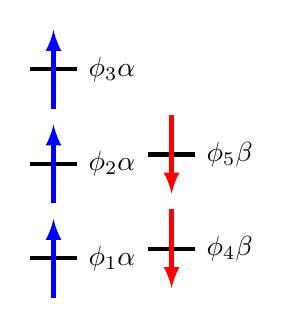
\begin{tikzpicture}[scale=0.6,
							upspinarrow/.pic = {\draw[-latex, blue] (0,-0.5) -- (0, 0.5);},
							downspinarrow/.pic = {\draw[latex-,red] (0,-0.5) -- (0, 0.5);}
						]
						\foreach \i[count=\xi] in {0,2,...,4}{ \draw[ultra thick]  (0,\i) -- pic[pos=0.5] {upspinarrow}   ++(1,0) node[right] {$\phi_{\xi}\alpha$};}
						\foreach \i[count=\xi from 4] in {0,2}{ \draw[ultra thick]  (2.5,\i+0.2) -- pic[pos=0.5] {downspinarrow}   ++(1,0) node[right] {$\phi_{\xi}\beta$};}
					\end{tikzpicture}
				\end{center}
				\onslide<2>
				\begin{center}
					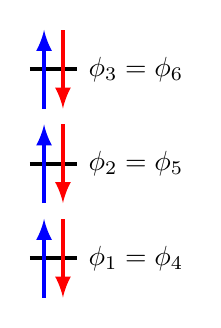
\begin{tikzpicture}[scale=0.6,
							upspinarrow/.pic = {\draw[-latex, blue] (0,-0.5) -- (0, 0.5);},
							downspinarrow/.pic = {\draw[latex-,red] (0,-0.5) -- (0, 0.5);}
						]
						\foreach \i[count=\xi, count=\yi from 4] in {0,2,...,4}{ \draw[ultra thick]  (0,\i) -- pic[pos=0.3] {upspinarrow}  pic[pos=0.7] {downspinarrow} (1,\i) node[right] {$\phi_{\xi} = \phi_{\yi}$};}
					\end{tikzpicture}
				\end{center}
			\end{overprint}
		\end{column}
		\begin{column}{0.7\linewidth}
			\begin{overprint}
				\onslide<1>
				\begin{equation*}\label{}
					\Phi_0 = \frac{1}{\sqrt{N_e}} \mathrm{det} \{\phi_1\alpha, \phi_2\alpha_2, \ldots, \phi_{N_\alpha +1}\beta, \ldots, \phi_{N}\beta\}
				\end{equation*}
				\begin{equation*}\label{}
					\hat{F}^{(\alpha)} = \hat{h} + \sum\limits_{j = 1}^{N_\alpha} \left(J_j - K_j\right) + \sum\limits_{j = N_\alpha + 1}^{N} J_j.
				\end{equation*}
				\begin{equation*}\label{}
					\hat{F}^{(\beta)} = \hat{h} + \sum\limits_{j = N_\alpha + 1}^{N} \left(J_j - K_j\right) + \sum\limits_{j =  1}^{N_\alpha} J_j.
				\end{equation*}
				\onslide<2>
				\begin{equation*}
					N_\alpha = N_\beta = N/2
				\end{equation*}
				\begin{equation*}\label{}
					\Phi_0 = \frac{1}{\sqrt{N_e}} \mathrm{det} \{\phi_1\alpha, \phi_2\alpha_2, \ldots, \phi_{N_\alpha +1}\beta, \ldots, \phi_{N}\beta\}
				\end{equation*}
				\begin{equation*}\label{}
					\phi_1 =  \phi_{N_\alpha +1}, \ldots, \phi_{N_\alpha} = \phi_N
				\end{equation*}
				Оператор Фока приймає вигляд
				\begin{equation*}\label{}
					\hat{F} = \hat{h} + \sum\limits_{j = 1}^{N/2} \left(2J_j - K_j\right).
				\end{equation*}
			\end{overprint}
		\end{column}
	\end{columns}
\end{frame}
%============================================================================

%============================================================================
\begin{frame}{Рівняння Хартрі-Фока}{Рівняння Хартрі-Фока-Рутаана}
	\begin{overprint}
		\onslide<1>
		Шукати функції в загальному вигляді, а тим більше тривимірні ніхто не вміє. Однак, якщо ми приймемо припущення, що нам доступний якийсь \alert{базисний набір} функцій $\chi_q$, то
		\begin{equation*}\label{}
			\phi_i(\vec{r}) = \sum\limits_{q = 1}^{N_b} c_{iq}\chi_q(\vec{r}).
		\end{equation*}
		причому $\chi_q(\vec{r})$ можуть бути неортогональними одна одній. При подібному фіксованому поданні задача пошуку форми орбіталей зводиться до пошуку $N_b$ коефіцієнтів представлення $c_{iq}$, а це вже не так страшно, хоча б зрозуміло що робити.
		\onslide<2>
		Далі підставляємо представлення в рівняння Хартрі-Фока:
		\begin{equation*}\label{}
			\hat{F}_i \sum\limits_{q = 1}^{N_b} c_{iq}\chi_q(\vec{r})\gamma_i = \varepsilon_i \sum\limits_{q = 1}^{N_b} c_{iq}\chi_q(\vec{r}).
		\end{equation*}
		після чого домножуємо обидві частини зліва на всі можливі інші комплексно-спряжені базисні функції $\chi_p^*\gamma_i$ і інтегруємо за координатами:
		\begin{equation*}\label{}
			\sum\limits_{q = 1}^{N_b} \opbracket{\chi_p}{\hat{F}_i}{\chi_q}\cdot c_{iq} = \varepsilon_i  \bracket{\chi_p}{\chi_q}\cdot c_{iq},
		\end{equation*}
		де $S_{pq} = \bracket{\chi_p}{\chi_q} = \int \chi_p^*(\vec{r}) \chi_q(\vec{r}) dr$~--- інтеграли перекривання базисних функцій.
		\onslide<3>
		\begin{equation*}\label{}
			\sum\limits_{q = 1}^{N_b}  c_{iq} \left(F_{pq} - \varepsilon_i   S_{pq} \right) = 0,  \quad p,q = 1,2,\ldots, N_b
		\end{equation*}
		або в матричній формі
		\begin{equation*}\label{}
			\tcbhighmath{\left(\mathcal{F}  - \varepsilon_i \mathcal{S}\right) \mathbf{c}_i = 0,}
		\end{equation*}
		отримали матричну задачу на пошук власних векторів \\ $\mathbf{c}_{i} = (c_{i1}, c_{i2}, \ldots, c_{iN_b})$ та власних значень $\varepsilon_i$ матриці $\mathcal{F}$.
		\\~\\
		Ці рівняння називаються \alert{рівняннями Хартрі-Фока-Рутаана}.
	\end{overprint}
\end{frame}
%============================================================================

%============================================================================
\begin{frame}{Рівняння Хартрі-Фока}{Елементи матриць: для методу RHF}
	\only<1-2>{%
		Матриця Фока
		\begin{equation*}\label{}
			F_{pq} = \opbracket{\chi_p}{\hat{F}}{\chi_q} = \opbracket{\chi_p}{\hat{h}}{\chi_q} + \sum\limits_{j = 1}^{N_e/2} 2 \opbracket{\chi_p}{\hat{J}_j}{\chi_q}  - \opbracket{\chi_p}{\hat{K}_j}{\chi_q}.
		\end{equation*}
	}%
	\only<3-4>{%
		Матриця Фока
		\begin{equation*}\label{}
			F_{pq} = \opbracket{\chi_p}{\hat{F}}{\chi_q} = \opbracket{\chi_p}{\hat{h}}{\chi_q} + \sum\limits_{r}^{N_b}\sum\limits_{s}^{N_b} P_{rs} \left[(pq|rs) - \frac12(ps|rq)\right].
		\end{equation*}
	}%
	\begin{overprint}
		\onslide<1>
		Кулонівський оператор\vspace*{-2ex}
		\begin{equation*}\label{}
			\hat{J}_j \chi_q = \chi_q(\vec{r}) \int \frac{\phi_j(\vec{r}')\phi_j(\vec{r}')}{r}d r' = \chi_q(\vec{r}) \sum\limits_{r}^{N_b}\sum\limits_{s}^{N_b} \int \frac{\chi_r(\vec{r}')\chi_s(\vec{r}')}{r}d r'.
		\end{equation*}
		Кулонівський інтеграл\vspace*{-2ex}
		\begin{multline*}\label{}
			\opbracket{\chi_p}{\hat{J}_j}{\chi_q} =   \sum\limits_{r}^{N_b}\sum\limits_{s}^{N_b}c^*_{rj}c_{sj} \int \frac{\chi_p^*(\vec{r})\chi_q(\vec{r}) \chi_r^*(\vec{r}')\chi_s(\vec{r}')}{r}dr d r' = \\[-1ex] = \sum\limits_{r}^{N_b}\sum\limits_{s}^{N_b}c^*_{rj}c_{sj} (pq|rs).
		\end{multline*}
		\onslide<2>
		Обмінний інтеграл\vspace*{-2ex}
		\begin{equation*}\label{}
			\opbracket{\chi_p}{\hat{K}_j}{\chi_q} =  \sum\limits_{r}^{N_b}\sum\limits_{s}^{N_b}c^*_{rj}c_{sj} (ps|rq).
		\end{equation*}
		\onslide<3>
		Введемо \alert{матрицю електронної густини}:
		\begin{equation*}\label{}
			P_{rs} =  2\sum\limits_{j = 1}^{N_e/2} c^*_{rj}c_{sj}.
		\end{equation*}
		Електронна густина
		\begin{equation*}\label{}
			\rho = 2 \sum\limits_{j=1}^{N_e/2} \phi_j^* \phi_j =  2\sum\limits_{j = 1}^{N_e/2} \sum\limits_{p = 1}^{N_b}\sum\limits_{q = 1}^{N_b} c^*_{pj}c_{qj} \chi_p\chi_q = \sum\limits_{p = 1}^{N_b}\sum\limits_{q = 1}^{N_b}  P_{pq}\chi_p\chi_q.
		\end{equation*}
		\onslide<4>
		Енергія
		\begin{equation*}\label{}
			E_\mathrm{HF} =  2\sum\limits_{i = 1}^{N_e/2} \varepsilon_i + \sum\limits_{p = 1}^{N_b}\sum\limits_{q = 1}^{N_b}  P_{pq}\opbracket{\chi_p}{\hat{h}}{\chi_q} + V_{nn},
		\end{equation*}
		$V_{nn}$~--- енергія міжядерного відштовхування.
	\end{overprint}
\end{frame}
%============================================================================

%============================================================================
\begin{frame}{Метод Хартрі-Фока}{Орбіталі слейтерівського типу (STO)}
	%----------------------------------------------------------------------------
	В якості базисних функцій для розрахунків використовують орбіталі слейтерівського типу  (STO), нормалізована форма яких має вигляд:
	\begin{equation*}
		\tcbhighmath{
		\chi_s = \frac{(2\zeta_s)^{n + 1/2}}{[(2n)!]^{1/2}} r^{n - 1}e^{-\zeta_s r} \cdot Y_{lm}(\theta, \phi).
		}
	\end{equation*}
	{\scriptsize \fullcite{Slater1930}}
	\begin{columns}
		\begin{column}{0.5\linewidth}
			\begin{center}
				\begin{tikzpicture}[]
					\begin{axis}[
							axis lines = middle,
							clip=false,
							ylabel={$\chi$},
							y label style={at={(axis description cs:-0.01,1)},anchor=east},
							xlabel={$r$}, x label style={at={(axis description cs:1,-0.01)},anchor=west},
							xmin=0, xmax=2.1,
							ymin=0, ymax=1.1,
							ticks=none,
							width = \linewidth,
							%y=1.7cm,
							%x=1cm,
						]

						\addplot[thick,
							domain=0:2, red, thick, samples=500,
						] {1*exp(-2*x)} node[black, pos=0.3,above,sloped] {$n = 1$};
						\addplot[thick,
							domain=0:2, blue, thick, samples=500,
						] {1*x*exp(-2*x)} node[black, pos=0.6,above,sloped] {$n = 2$};

					\end{axis}
				\end{tikzpicture}
			\end{center}
		\end{column}
		\begin{column}{0.5\linewidth}
			\begin{overprint}
				\onslide<1>
				Орбітальна експонента $\zeta$:
				\[\zeta = \frac{Z-\sigma}{n}\]
				де
				$Z$ --  заряд ядра,\\
				$\sigma$ -- константа екранування,\\
				$n$ -- ефективне квантове число.
				\onslide<2>
				Радіальні частини STO не мають вузлів і задовольняють асимптотичній поведінці точної хвильової функції поблизу ядра та на великих відстанях від нього. При $l = n - 1$ \texttt{STO} переходить в АО воднеподібного атома.
			\end{overprint}
		\end{column}
	\end{columns}
	%----------------------------------------------------------------------------
\end{frame}
%============================================================================




%============================================================================
\begin{frame}{Орбіталі гаусового типу (GTO)}
	%----------------------------------------------------------------------------
	\begin{onlyenv}<1>
		{{\scriptsize Про базиси \fullcite[Глава 14, \S 14.1]{Sleta} або \fullcite[Chapter 15, 15.4]{Levine}}}

		\begin{itemize}
			\item Для \alert{атомних розрахунків} цілком достатньо використовувати в якості базисних функцій слейтерівькі орбіталі (STO), параметри $\zeta$ цих орбіталей затабульовані.

			      {\scriptsize [\fullcite{ClementiRoetti}]}

			\item При проведенні \alert{молекулярних розрахунків}, взяття інтегралів (елементи матриці Фока, та матриці перекриття) із-за наявності фактора $e^{-\zeta r}$ становить математичні труднощі.
		\end{itemize}

		{\scriptsize В якості базисних функцій використовувати орбіталі, в яких замість фактора $e^{-\zeta r}$ вводиться $e^{-\alpha r^2}$, такі орбіталі називаються орбіталі гаусового типу GTO (gaussian-type orbitals) [\fullcite{Boys}]}
		%----------------------------------------------------------------------------
	\end{onlyenv}
	\begin{onlyenv}<2>
		Орбіталі гаусового типу мають вигляд:
		\begin{equation*}\label{GTO}
			\tcbhighmath{%
				\mathrm{GTO}(x,y,z;\alpha,i,j,k) = \left(\frac{2\alpha}{\pi}\right)^{3/4}\sqrt{\frac{(8\alpha)^{i + j + k} i!j!k!}{(2i)!(2j)!(2k)!}} x^{i} y^{j} z^{k} e^{-\alpha r^2}
			}
		\end{equation*}

		\begin{itemize}
			\item при $i + j + k = 0$ (тобто, коли $i = 0$, $j = 0$, $k = 0$) GTO називаються $s$-типу;
			\item при $i + j + k = 1$ ми маємо GTO $p$-типу;
			\item при $i + j + k = 2$ ми маємо GTO $d$-типу;
			\item ...
		\end{itemize}

		{\scriptsize Існує шість GTO $d$-типу, з множниками $x^2$, $y^2$, $z^2$, $xy$, $xz$ та $yz$. П’ять лінійних комбінацій (множники $xy$, $xz$, $yz$, $x^2 - y^2$ і $3z^2 - r^2$) можна утворити так, щоб вони мали однакову куту поведінка як п'ять реальних $3d$ AO; шоста комбінація з множником $x^2 + y^2 + z^2 = r^2$ подібна функції $3s$. Ця шоста комбінація часто опускається з базового набору.}

		%Notice that the difference between the STO and GTO is in the $r$-expotetnt The GTO squares the $r$ so that the product of the gaussian <<primitives>> (original gaussian equations) is another gaussian. By doing this, we have an equation we can work with and so the equation is much easier. However, the price we pay is loss of accuracy. To compensate for this loss, we find that the more gaussian equations we combine, the more accurate our equation.
		%
		%All basis set equations in the form STO-nG (where n represents the number of GTOs combined to approximate the STO) are considered to be <<minimal>> basis sets. The <<extended>> basis sets, then, are the ones that consider the higher orbitals of the molecule and account for size and shape of molecular charge distributions.
	\end{onlyenv}

	%----------------------------------------------------------------------------
\end{frame}
%============================================================================





%============================================================================
\tikzstyle{every picture}+=[remember picture]
\begin{frame}{Базисні функції 1s-STO та 1s-GTO}
	%----------------------------------------------------------------------------
	\(
	\underbrace{\tcbhighmath[drop fuzzy shadow, colframe=cyan]{\phi_{STO} =  \left( \frac{\zeta}{\pi}\right)^{1^{}/2} e^{-\zeta r}}}_{ST\tikzmark{1}O}
	\)
	\hfill
	\(
	\underbrace{\tcbhighmath[drop fuzzy shadow]{\phi_{GTO} =  \left( \frac{2\alpha}{\pi}\right)^{3^{}/4} e^{-\alpha r^2}}}_{GT\tikzmark{2}O}
	\)

	\begin{center}
		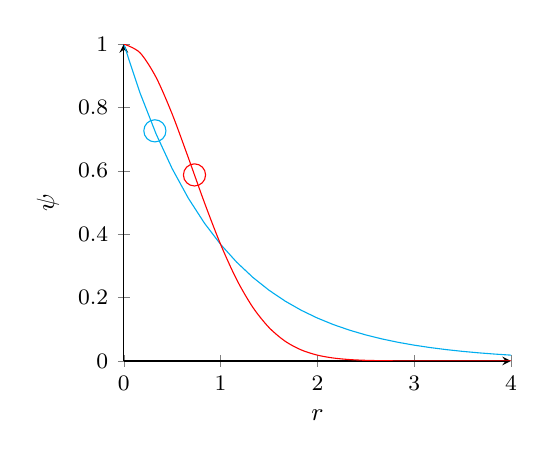
\begin{tikzpicture}[
				remember picture,
			]
			\begin{axis}[
					axis lines=left,
					xlabel=$r$,
					ylabel=$\psi$,
					small,
				]

				\addplot [cyan, domain={0:4}]
				{1*exp(-x)} node [pos=0.1] (n1) {};


				\addplot [red, domain={0:4}, smooth]
				{1*exp(-x^2)} node [pos=0.2] (n2) {};

				%            \fill<1-> [cyan] (n1) circle (2pt);
				%            \fill<2-> [red]  (n2) circle (2pt);

			\end{axis}

			% for debugging purposes only
			\draw [cyan] (n1) circle (4pt);
			\draw [red]  (n2) circle (4pt);
		\end{tikzpicture}
	\end{center}

	\begin{tikzpicture}[
			remember picture,
			overlay,
			arrows={-Latex},
			ultra thick,
		]
		\draw[bend left=45, cyan] (n1) to (pic cs:1);
		\draw[bend right=45,red] (n2) to (pic cs:2);
	\end{tikzpicture}
	%----------------------------------------------------------------------------
\end{frame}
%============================================================================





%============================================================================
\begin{frame}{Недоліки GTO. Контрактація базису}
	%----------------------------------------------------------------------------
	\begin{itemize}
		\item Поведінка GTO не схожа на справжню поведінка АО поблизу ядра, і швидко спадає на нескінченності (на відміну від STO).
		\item Якщо Взяти достатню кількість GTO, можна апроксимувати STO.
	\end{itemize}

	\begin{equation*}
		\tcbhighmath[drop fuzzy shadow]{
			\mathrm{STO} \approx  \sum \mathrm{GTO} ,
		}
	\end{equation*}
	Набір GTO що апроксимують STO --- називається \alert{стисненням}, або \alert{контрактацією} базису.

	\medskip

	{\scriptsize Базиси  STO-NG, де $N$ --- число гаусових функцій (GTO), які \alert{стискують} (\alert{контрактують}) одну орбіталь STO називають \alert{мінімальним базисом}. Під терміном \alert{мінімальний базис} розуміють базисний набір, при якому \alert{число базисних функцій атома визначається числом заповнених оболонок атома}.}
	%    {\small Функції GTO називаються примітивними гаусовими функціями, або примітивами, і таких функцій потрібно істотно більше, ніж STO, але це з лишком компенсується аналітичними виразами для інтегралів.}
	%----------------------------------------------------------------------------
\end{frame}
%============================================================================





%============================================================================
\begin{frame}{Приклад контрактації STO-3G}
	%----------------------------------------------------------------------------
	\begin{equation*}\footnotesize
		\text{STO-3G} =
		\highlight{cyan!50}{c_1 \cdot  \left(\frac{2\alpha_1}{\pi}\right)^{3/4}e^{-\alpha_1r^2}}{ge1}
		+
		\highlight{magenta!50}{%
		c_2 \cdot  \left(\frac{2\alpha_2}{\pi}\right)^{3/4}e^{-\alpha_2r^2}}{ge2}
		+
		\highlight{green!50}{%
		c_3 \cdot \left(\frac{2\alpha_3}{\pi}\right)^{3/4}e^{-\alpha_3r^2}}{ge3}
	\end{equation*}

	\begin{center}
		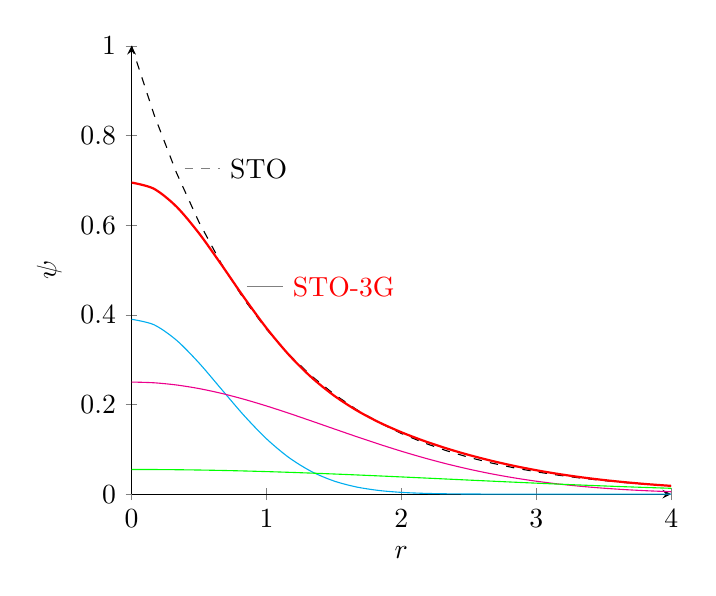
\begin{tikzpicture}[remember picture]
			\begin{axis}[
					axis lines=left,
					xlabel=$r$,
					ylabel=$\psi$,
				]
				\newcommand{\es}{0.39*exp(-1.15*x^2)}
				\newcommand{\p}{0.25*exp(-0.24*x^2)}
				\newcommand{\de}{0.055*exp(-0.09*x^2)}
				\addplot [dashed, domain={0:4}]
				{1*exp(-x)} node [pos=0.1, pin=0:STO] (s1) {};


				\addplot [cyan, domain={0:4}, smooth]
				{\es} node [pos=0.1] (g1) {};

				\addplot [magenta, domain={0:4}, smooth]
				{\p} node [pos=0.2] (g2) {};

				\addplot [green, domain={0:4}, smooth]
				{\de} node [pos=0.2] (g3) {};

				\addplot [thick, domain={0:4}, smooth, red]
				{\es + \p +\de} node [pos=0.2, pin=0:STO-3G] (gs) {};

			\end{axis}
		\end{tikzpicture}
	\end{center}

	\begin{tikzpicture}[
			%remember picture,
			overlay,
			arrows={-Latex},
		]
		%\draw<2>[]     (s1) to (pic cs:ge1);
		\draw[cyan] (g1) edge (ge1);
		\draw[magenta]  (g2) edge (ge2);
		\draw[green]  (g3) edge (ge3);
	\end{tikzpicture}
	%----------------------------------------------------------------------------
\end{frame}
%============================================================================





%============================================================================
\begin{frame}{Рівняння Хартрі-Фока}{Алгоритм розв'язку}
	\begin{tikzpicture}[scale=0.5, every node/.style={scale=0.5},
			info/.style={font=\small\ttfamily, text width=5cm},
			tharrow/.style={thick, arrows=-stealth},
			startstop/.style={rectangle, rounded corners, text width=5cm,  text centered, draw=black, fill=red!30},
			var/.style={rectangle, rounded corners, text width=2cm,  text centered, draw=black, fill=green!30},
			process/.style={rectangle, text width=6cm, minimum height=1cm, text centered, draw=black, fill=orange!30},
			io/.style={trapezium, trapezium left angle=70, trapezium right angle=110, text width=4.7cm, text centered, draw=black, fill=blue!30},
			decision/.style={diamond,  aspect=3, text width=4cm, text centered, draw=black, fill=yellow!30},
		]
		\def\internode{10pt}
		\node (basis) [io]  {$\{\chi_q(\vec{r})\}$}; \node[right=12pt of basis, info] {Вибір базисних функцій};
		\node (n0) [var, below = \internode of basis] {$n = 0$};
		\node (coeff) [startstop,below = \internode of n0] {$c^{(n)}_{kq}$}; \node[right=12pt of coeff, info] {Вибір початкових коефіцієнтів};
		\node (integ) [process,below = \internode of coeff]   {$P^{(n)}_{pq}$, $F^{(n)}_{pq}$}; \node[right=5pt of integ, info] {Обчислення інтегралів та формування матриць};
		\node (HFR)   [process,below = \internode of integ]   {$\sum\limits_{q = 1}^{N_b}  c^{(n + 1)}_{kq} \left(F^{(n)}_{pq} - \varepsilon^{(n + 1)}_k   S_{pq} \right) = 0$};  \node[right=5pt of HFR, info] {Розв'язок рівнянь Хартрі-Фока};
		\node (Energy) [process,below =\internode of HFR]  { $E^{(n + 1)} =  2\sum\limits_{i = 1}^{N_e/2} \varepsilon_i^{(n+1)} + \sum\limits_{p = 1}^{N_b}\sum\limits_{q = 1}^{N_b}  P^{(n)}_{pq}\opbracket{\chi_p}{\hat{h}}{\chi_q} + V_{nn}$}; \node[right=5pt of Energy, info] {Розрахунок енегрії};
		\node (Condition) [decision,below = \internode of Energy] {$|E^{(n + 1)} - E^{(n)}| \le \delta $};
		\node (output) [io, right = 10pt of Condition] {Властивості};
		\node (n1) [var, left = 10pt of HFR] {$n\,\, +\kern-1ex= 1$};
		\draw [tharrow] (basis) -- (n0) ;
		\draw [tharrow] (n0) -- (coeff) ;
		\draw [tharrow] (coeff) -- (integ);
		\draw [tharrow] (integ) -- (HFR);
		\draw [tharrow] (HFR) -- (Energy);
		\draw [tharrow] (Energy) -- (Condition);
		\draw [tharrow] (Condition.west)  -| node[above, pos=0.25] {0} (n1)  |- (coeff.west);
		\draw [tharrow] (Condition.east) -- node[above, pos=0.25] {1} (output);
	\end{tikzpicture}
\end{frame}
%============================================================================





%============================================================================
\begin{frame}{Висновки}{Переваги та недоліки методі Хартрі-Фока}

	%        Метод використовує наближення незалежних частинок, а електронну взаємодію враховує як суму взаємодій кожного електрона із середньою електронною густиною інших електронів.
	%        Насправді, між усіма електронами існує миттєве кулонівське відштовхування, тобто. їхній рух корельований.

	\begin{enumerate}[\faHandORight]
		\item Метод Хартрі-Фока дозволяє відносно добре описувати стан молекулярних систем поблизу їх стійких (рівноважних) конфігурацій, що відповідають точкам мінімуму на поверхнях потенціальної енергії основного електронного стану,
		\item Дає некоректні оцінки енергій дисоціації, енергетичних бар'єрів, що відповідають перетворенню однієї стійкої молекулярної форми на іншу.
		\item Не дозволяє він розглядати збуджені електронні стани молекул.
	\end{enumerate}

\end{frame}
%============================================================================

%============================================================================
%\begin{frame}{Рівняння Хартрі-Фока}{Алгоритм розв'язку для атома гелію}\footnotesize
%	Базисні функції
%	\begin{equation*}\label{}
%		\chi_1 = \frac1{\sqrt{4\pi}}2\zeta_1^{3/2}e^{-\zeta_1r}, \quad \chi_2 = \frac1{\sqrt{4\pi}}2\zeta_1^{3/2}e^{-\zeta_2r}, \zeta_1 = 1.45, \quad \zeta_2 = 2.91.
%	\end{equation*}
%	\begin{overprint}
%		\onslide<1>
%		Компоненти матриці перекривання
%		\begin{equation*}\label{}
%			S_{11} = S_{22} = 1, \quad S_{12} = S_{21} = \frac{8\zeta_1^{3/2} \zeta_2^{3/2}}{(\zeta_1 + \zeta_2)^3} = 0.8366
%		\end{equation*}
%
%		Компоненти $\opbracket{\chi_p}{\hat{h}}{\chi_q}$
%		\begin{align*}\label{}
%			\opbracket{\chi_1}{\hat{h}}{\chi_1} = -\frac12\zeta_1^{3/2} + (\zeta_1 - 2)\zeta_1 = -1.8488, \quad \opbracket{\chi_2}{\hat{h}}{\chi_2} = -1.5860 \\
%			\opbracket{\chi_1}{\hat{h}}{\chi_2} = \opbracket{\chi_2}{\hat{h}}{\chi_1} = \frac{\zeta_1^{3/2}\zeta_2^{3/2}(4\zeta_1\zeta_2 - 8(\zeta_1 + \zeta_2))}{(\zeta_1 + \zeta_2)^3} = -1.8826.
%		\end{align*}
%		\onslide<2>
%		Кулонівські та обмінні інтеграли
%		\begin{align*}\label{}
%			(11|11) & = \frac58\zeta_1 = 0.9062, \quad (22|22) = \frac58\zeta_2 = 1.8188,                                                           \\
%			(11|22) & = (22|11) = (\zeta_1^4\zeta_2 + 4\zeta_1^3\zeta_2^2 + \zeta_1\zeta_2^4 + 4\zeta_1^2\zeta_2^3)/(\zeta_1 + \zeta_2)^4 = 1.1826, \\
%			(12|12) & = (21|12) = (12|21) = (21|21) = 20\zeta_1^3\zeta_2^3/(\zeta_1 + \zeta_2)^5 = 0.9535,                                          \\
%			(11|12) & = (11|21) = (12|11) = (21|11) =                                                                                               \\ &= \frac{16\zeta_1^{9/2}\zeta_2^{3/2}}{(3\zeta_1 + \zeta_2)^4}\left[\frac{12\zeta_1 + 8\zeta_2}{(\zeta_1 + \zeta_2)^2} + \frac{9\zeta_1 + \zeta_2}{2\zeta_1^2}\right] = 0.9033,\\
%			(12|22) & = (22|12) = (21|22) = (22|21) = 1.2980.
%		\end{align*}
%		\onslide<3>
%		Для вибору початкових коефіцієнтів візьмемо співвідношення $c_{11}/c_{21} \approx 2 = k$ . \\~\\
%		Умова нормування $\int |\phi_1|^2 dv = \int (c_{11}\chi_1 + c_{21}\chi_2)^2 dv = 1$ дає співвідношення $c_{21} = \sqrt{1 + k^2 + 2kS_{12}} \approx  0.3461$, $c_{11} = 0.6922$.\\~\\
%		Елементи матриці густини:
%		\begin{align*}\label{}
%			P_{11} = 2c_{11}c_{11} \approx 0.9583, \quad P_{12} = 2c_{11}c_{12} \approx 0.4791, \\
%			P_{21} = 2c_{21}c_{11} \approx 0.4791, \quad P_{22} = 2c_{21}c_{21} \approx 0.2396.
%		\end{align*}
%		\onslide<4>
%		Елементи матриці Фока:
%		\begin{align*}\label{}
%			F_{11} & = h_{11} + \frac12P_{11}(11|11) +  P_{12}(11|12) +P_{22}\left[(11|22) - \frac12(12|21)\right],              \\
%			F_{12} & = h_{12}+ \frac12P_{11}(12|11) + P_{12}\left[\frac32(12|12) - \frac12(11|22)\right] + \frac12P_{22}(12|22), \\
%			F_{22} & = F_{12},                                                                                                   \\
%			F_{22} & = h_{22} + P_{11}\left[(22|11) - \frac12(21|12)\right] + P_{12}(22|12) + \frac12P_{22}(22|22).
%		\end{align*}
%		\onslide<5>
%		Елементи матриці Фока:
%		\begin{align*}\label{}
%			F_{11} & = -1.8448 + 0.4531P_{11} +0.9033P_{12} + 0.7058P_{22},          \\
%			F_{12} & = F_{12} = -1.8826 + 0.45165P_{11} + 0.8391P_12 + 0.6490P_{22}, \\
%			F_{22} & = -1.5860 + 0.7058P_{11} + 1.2980P_{12} + 0.9094P_{22}.
%		\end{align*}
%		\begin{equation*}\label{}
%			F_{11} \approx -0.813, \quad F_{12} = F_{12} \approx -0.892, \quad F_{22} \approx -0.070\\
%		\end{equation*}
%		\onslide<6>
%		Розв'яжемо секулярне рівняння $\mathrm{det}(F_{pq} - S_{pq}\varepsilon_i) = 0$
%		\begin{equation*}\label{}
%			\left|
%			\begin{matrix}
%				-0.813 - \varepsilon_i       & -0.892 - 0.8366\varepsilon_i \\
%				-0.892 - 0.8366\varepsilon_i & -0.070-\varepsilon_1
%			\end{matrix}
%			\right| \approx 0.
%		\end{equation*}
%		\begin{equation*}\label{}
%			0.3001\varepsilon_1^2 - 0.6095\varepsilon_i - 0.739 \approx 0
%		\end{equation*}
%		\begin{equation*}\label{}
%			\varepsilon_1 \approx -0.854, \quad \varepsilon_2 \approx 2.885
%		\end{equation*}
%		\onslide<7>
%		Вибираємо корінь з меншою енергією і підставляємо його в рівняння Хартрі-Фока-Рутаана з  $p = 2$.
%		\begin{equation*}\label{}
%			c_{11}(F_{21} - \varepsilon_1S_{21}) + c_{21}(F_{22} - \varepsilon_1S_{22}) \approx 0.
%		\end{equation*}
%		\begin{equation*}\label{}
%			-0.1775 c_{11}  + 0.784 c_{21} \approx 0.
%		\end{equation*}
%		\begin{equation*}\label{}
%			c_{11}/c_{21} \approx 4.42.
%		\end{equation*}
%		Отримуємо поправлені коефіцієнти $c_{12} = 0.189$, $c_{11} = 0.836$.
%	\end{overprint}
%\end{frame}
%============================================================================

\end{document}
